\documentclass[12pt]{article}
 
\usepackage[margin=1in]{geometry} 
\usepackage{amsmath,amsthm,amssymb}
\usepackage{hyperref}
\usepackage{graphicx}
\usepackage{xcolor}
\usepackage[many]{tcolorbox}
\tcbuselibrary{listings}
\usepackage{listings}

\definecolor{lg}{HTML}{f0f0f0}

\newtcblisting{pycode}{
    colback=lg,
    boxrule=0pt,
    arc=0pt,
    outer arc=0pt,
    top=0pt,
    bottom=0pt,
    colframe=white,
    listing only,
    left=15.5pt,
    enhanced,
    listing options={
        basicstyle=\small\ttfamily,
        keywordstyle=\color{blue},
        language=Python,
        showstringspaces=false,
        tabsize=2,
        numbers=left,
        breaklines=true
    },
    overlay={
        \fill[gray!30]
        ([xshift=-3pt]frame.south west)
        rectangle
        ([xshift=11.5pt]frame.north west);
    }
}

\lstset{
    language=Python,
    basicstyle=\small\ttfamily,
}

 
\begin{document}
 
\title{Exercise 6}
\author{Jari Mattila - 35260T\\
ELEC-E8125 - Reinforcement Learning}

\maketitle

\section*{Task 1}

Revisit the policy gradient solution for the continuous Cartpole from
Exercise 5 with learned sigma and implement the actor-critic algorithm. 
In the initial setup, perform TD(0) updates at the end of each episode.
\newline

The training performance plots for each of the tasks (Tasks 1, 2 and 3).
\newline

\noindent
Source files: cartpole.py, agent\_task1a.py, agent\_task1b.py, agent\_task1c.py 

\section*{Question 1}

What is the relationship between actor-critic and REINFORCE with
baseline?

\section*{Question 2}

How can the value of advantage be intuitively interpreted?

\section*{Task 2}

Update the actor-critic code to perform TD(0) updates every 50 timesteps,
instead of updating your network at the end of each episode. Make sure to handle the end of
each episode correctly (as in the previous exercises, the value of the terminal state is 0).
\newline

The training performance plots for each of the tasks (Tasks 1, 2 and 3).
\newline

\noindent
Source files: cartpole.py, agent\_task1a.py, agent\_task1b.py, agent\_task1c.py 

\section*{Task 3}

Update your code to use parallel data collection. Start up with the
parallel\_cartpole.py script. This code makes use of the parallel wrapper for the environment,
which can be found in parallel\_env.py. This code instantiates processes worker processes,
with envs\_per\_process threads each. After adapting your code, run it with at least 20 parallel
environments and report the results. You can use Aalto computational resources (Maari,
Paniikki) if your computer runs sluggish.
\newline

The training performance plots for each of the tasks (Tasks 1, 2 and 3).
\newline

\noindent
Source files: cartpole.py, agent\_task1a.py, agent\_task1b.py, agent\_task1c.py 

\section*{Question 3}

How is parallel data collection different from the parallelism in
multiple\_cartpoles.py script we’ve seen in Exercises 1 and 5? Can it replace multiple runs of
the training algorithm for comparing RL algorithms? \textbf{Explain your answer.}

\section*{Question 4}

Figure 1 shows the training performance for all three actor-critic
variants and the REINFORCE algorithm from the last lecture. In terms of initial performance,
REINFORCE seems to completely outperform all tested A2C flavours on Cartpole, despite being
a simpler algorithm. \textbf{Why is it so? Explain your answer.}

\section*{Question 5.1}

How do actor-critic methods compare to REINFORCE in terms of
bias and variance of the policy gradient estimation? \textbf{Explain your answer.}

\section*{Question 5.2}

How could the bias-variance tradeoff in actor-critic be controlled?

\section*{Question 6}

What are the advantages of policy gradient and actor-critic methods
compared to action-value methods such as Q-learning? \textbf{Explain your answer.}



\pagebreak


\section{Question 1}

If you add a figure, you can refer to it using Figure.~\ref*{fig:fig1}.

\begin{figure}[h] 
	\centering  % Remember to centre the figure
    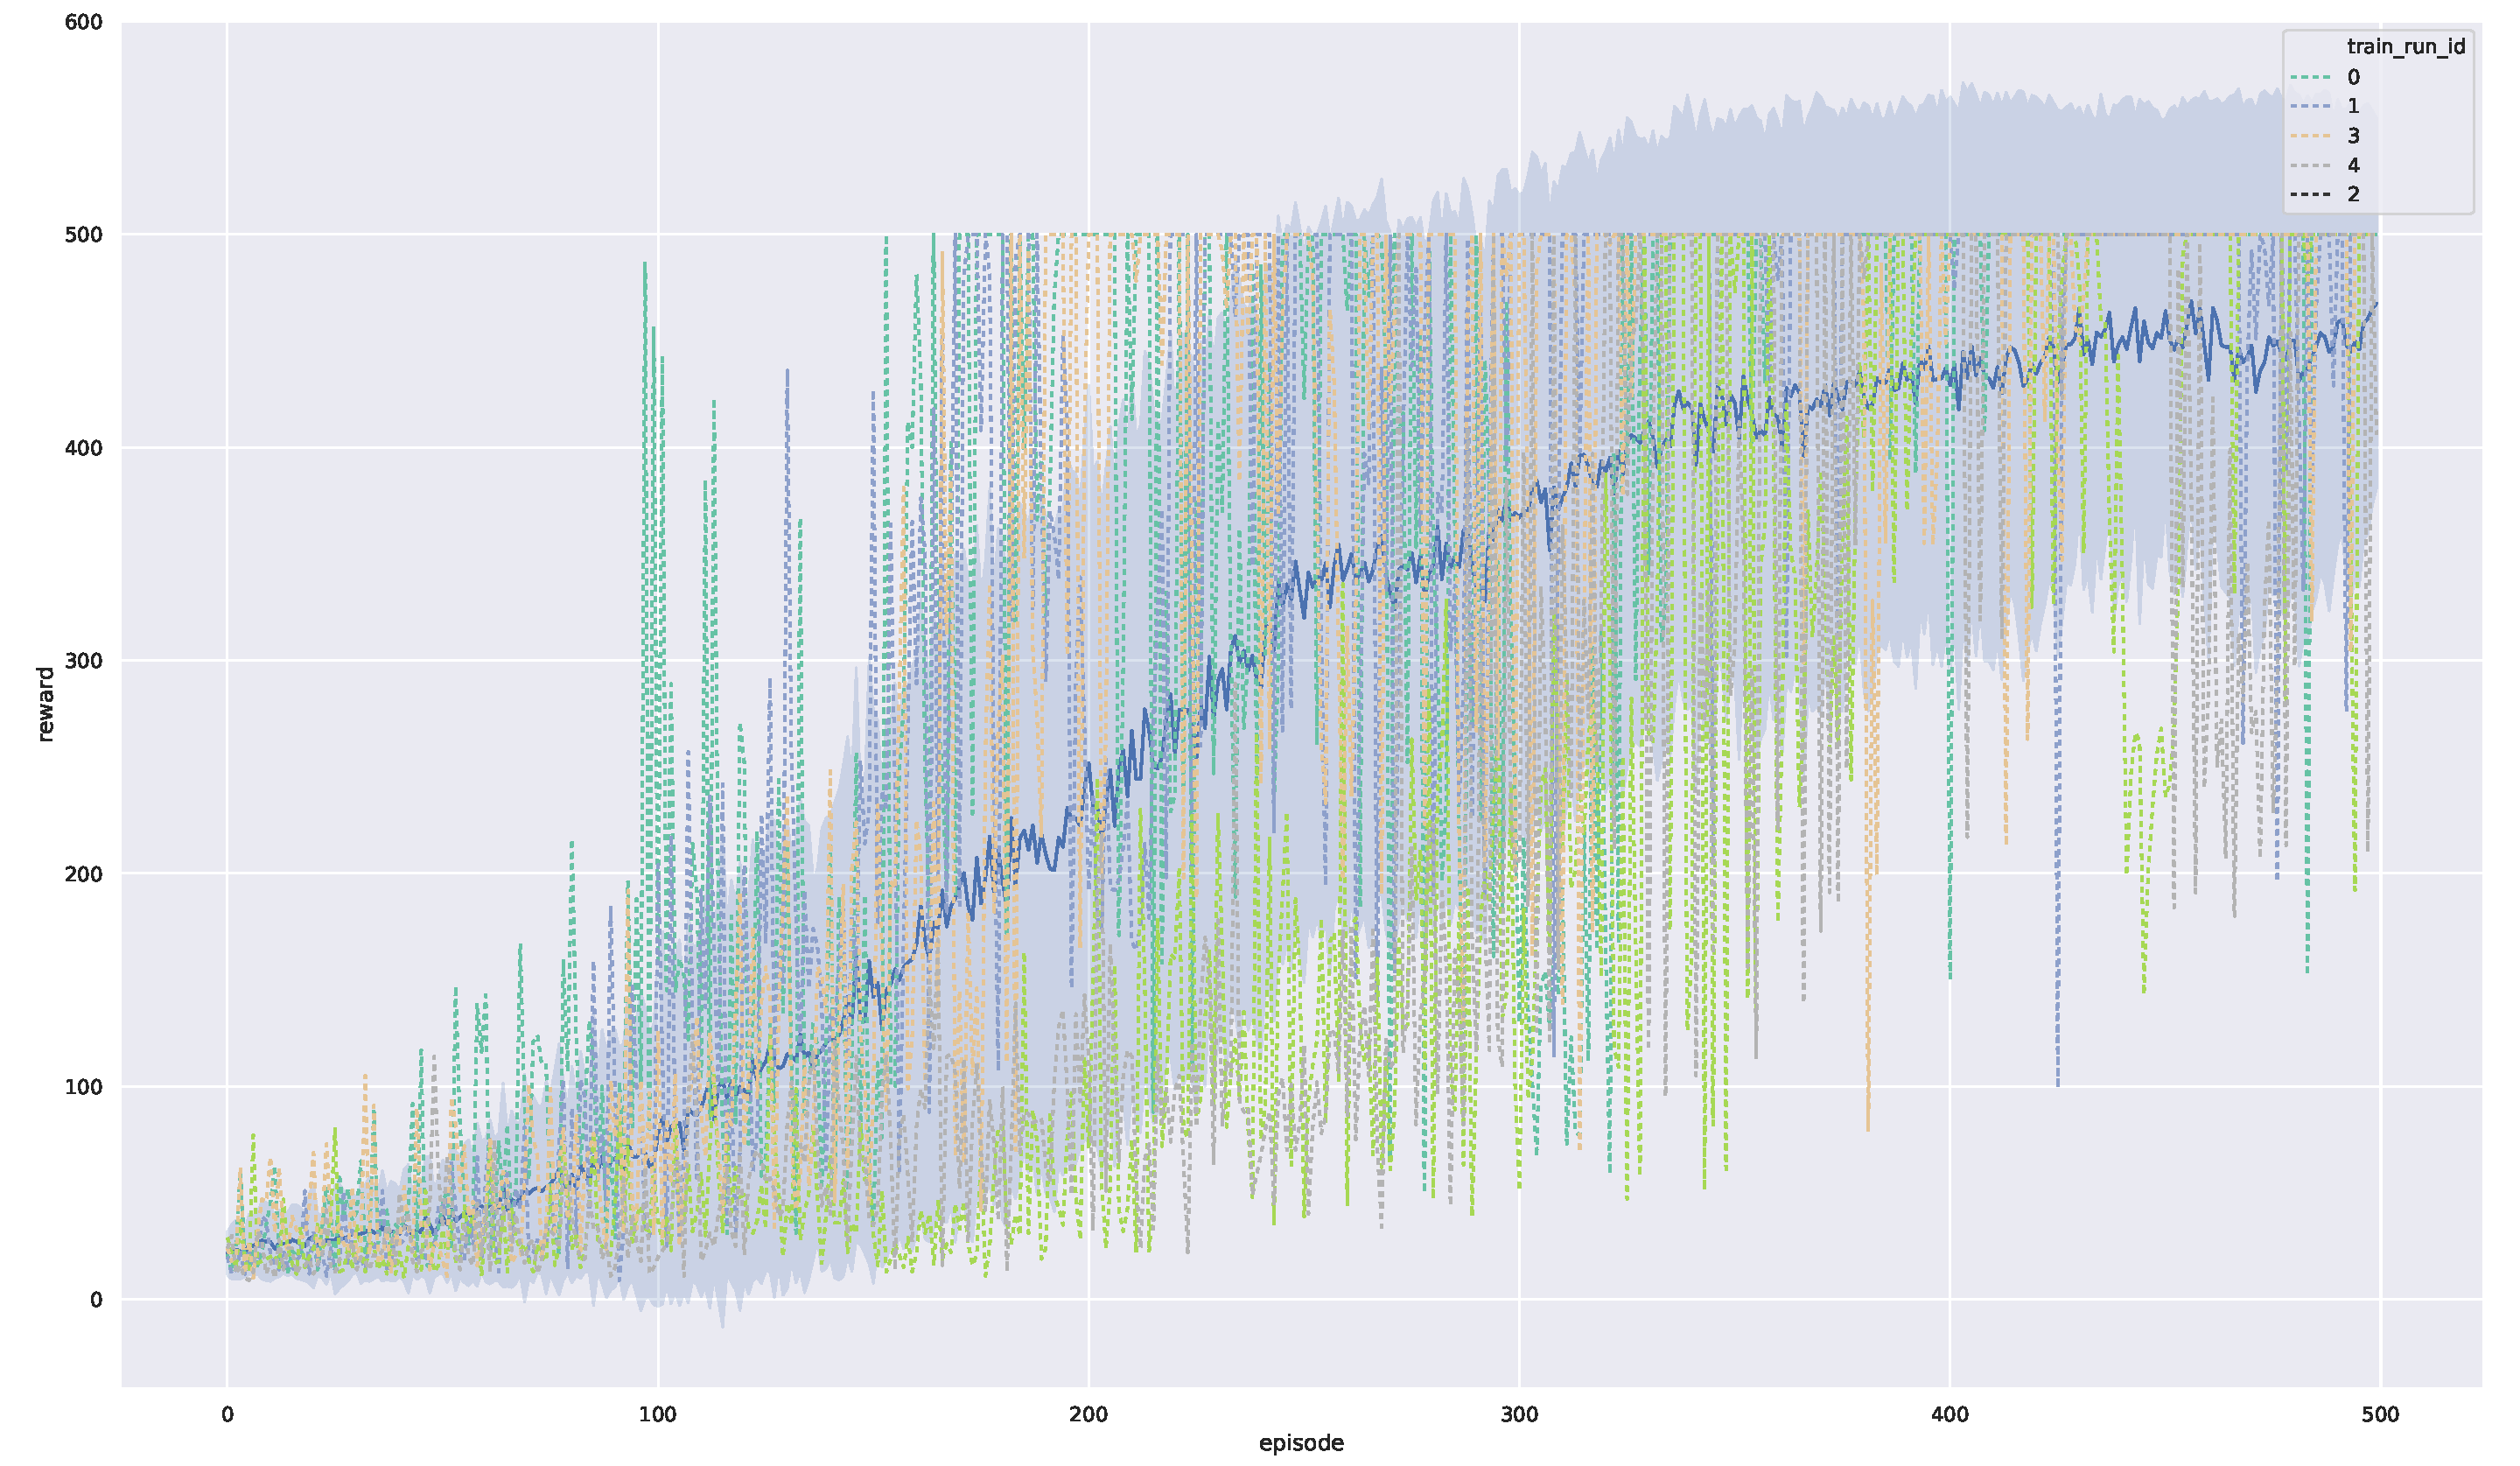
\includegraphics[width=0.9\columnwidth]{img/training.pdf}
	\caption{This is a sample figure.}
	\label{fig:fig1}
\end{figure}

\bibliographystyle{ieeetr}
\bibliography{template}  % Modify template with your bibliography name
\end{document}
